\documentclass[12pt,letterpaper]{article}
\usepackage[utf8]{inputenc}
\usepackage{amsmath,amssymb,fullpage,graphicx}
\usepackage{subfigure}
\let\hat\widehat
\let\tilde\widetilde


\author{Nan Tang\\1662478}
	%% your name
\title{STAT 403 Spring 2018\\HW05}
	%% title of this document
\begin{document}
\maketitle
	%% make the title and author

\section*{Q1}
\subsection*{Q1-a}
\begin{verbatim}
bern_p <- function(x) {
  return(exp(1 + 2 * x) / (1 + exp(1 + 2 * x)))
}
n <- 500
x_value <- runif(n)
y_value <- rbinom(n, size=1, p=bern_p(x_value))
xy_logic = glm(y_value~x_value, family = "binomial")

beta0 <- summary(xy_logic)$coefficient[1,1]
beta1 <- summary(xy_logic)$coefficient[2,1]

> beta0
[1] 1.029713
> beta1
[1] 2.025165
\end{verbatim}

\noindent In one time simulation under sample size 500, $\hat{beta}_1$ and $\hat{\beta}_0$ are respectively 2.0251 and 1.0297.

\newpage
\subsection*{Q1-b}
\begin{verbatim}
N = 2000
beta0_sim <- rep(NA, N)
beta1_sim <- rep(NA, N)

for (ii in 1:N) {
  x_value <- runif(n)
  y_value <- rbinom(n, size=1, p=bern_p(x_value))
  xy_logic = glm(y_value~x_value, family = "binomial")
  beta0_sim[ii] <- summary(xy_logic)$coefficient[1,1]
  beta1_sim[ii] <- summary(xy_logic)$coefficient[2,1]
}

hist(beta0_sim, probability=T, main='Histogram of Fitted Beta0', breaks=20,
     xlab='Fitted Beta0', col='coral1')
abline(v=1, lwd=3, col='cornflowerblue' )
legend('topright', 'True Beta0', col='cornflowerblue', lwd=3, cex=0.75)

\end{verbatim}

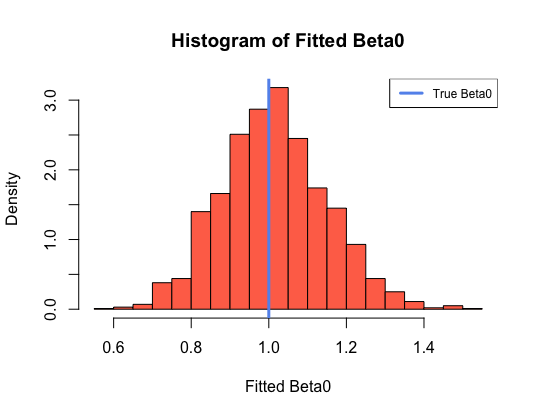
\includegraphics[width=150mm]{hist_beta0.png}

\begin{verbatim}
hist(beta1_sim, probability=T, main='Histogram of Fitted Beta1', breaks=20,
     xlab='Fitted Beta1', col='cornflowerblue')
abline(v=2, lwd=3, col='coral1' )
legend('topright', 'True Beta1', col='coral1', lwd=3, cex=0.75)
\end{verbatim}

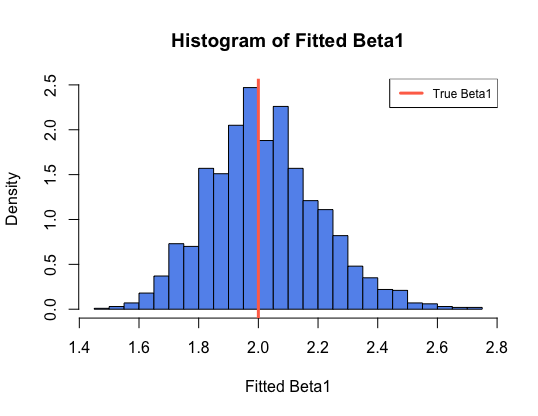
\includegraphics[width=150mm]{hist_beta1.png}

\subsection*{Q1-c}
\noindent From previous histograms describing the distributions, we can perceive that $\hat{\beta}_0$ and $\hat{\beta}_1$ both follow normal distribution. 

\newpage
\subsection*{Q1-d}
\begin{verbatim}
n = 2000
beta0_sim <- rep(NA, N)
beta1_sim <- rep(NA, N)
for (ii in 1:N) {
  x_value <- runif(n)
  y_value <- rbinom(n, size=1, p=bern_p(x_value))
  xy_logic = glm(y_value~x_value, family = "binomial")
  beta0_sim[ii] <- summary(xy_logic)$coefficient[1,1]
  beta1_sim[ii] <- summary(xy_logic)$coefficient[2,1]
}

hist(beta0_sim, probability=T, main='Histogram of Fitted Beta0', breaks=20,
     xlab='Fitted Beta0', col='coral1', xlim=c(0.2, 1.8))
abline(v=1, lwd=3, col='cornflowerblue' )
legend('topright', 'True Beta0', col='cornflowerblue', lwd=3, cex=0.75)
\end{verbatim}

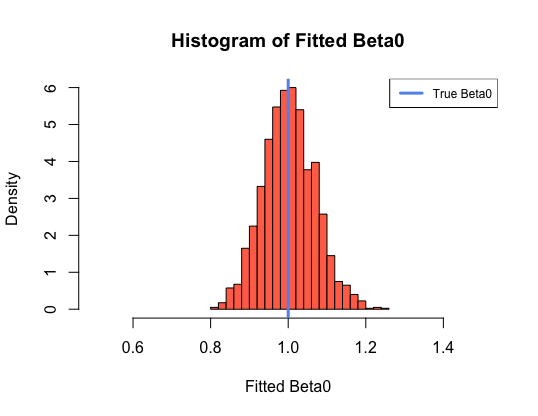
\includegraphics[width=150mm]{hist_beta0_2.png}

\begin{verbatim}
hist(beta1_sim, probability=T, main='Histogram of Fitted Beta1', breaks=20,
     xlab='Fitted Beta1', col='cornflowerblue', xlim=c(0.5, 4.0))
abline(v=2, lwd=3, col='coral1' )
legend('topright', 'True Beta1', col='coral1', lwd=3, cex=0.75)
\end{verbatim}

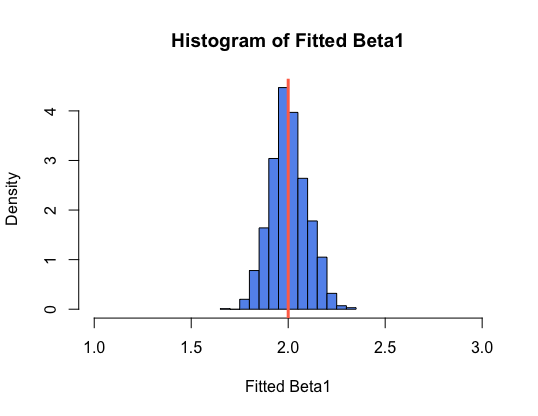
\includegraphics[width=150mm]{hist_beta1_2.png}

\noindent Both distributions concentrate more around true parameters, compare to sample size 500.


\subsection*{Q1-e}
\begin{verbatim}
library(Metrics)
sample_sizes <- seq(from=100, to=2000, by=200)
beta1_mse <- rep(NA, length(sample_sizes))
N = 2000

for (ii in 1:length(sample_sizes)) {
  n <- sample_sizes[ii]
  beta1 <- rep(NA, N)
  for (jj in 1:N) {
    x_value <- runif(n)
    y_value <- rbinom(n, size=1, p=bern_p(x_value))
    xy_logic = glm(y_value~x_value, family = "binomial")
    beta1[jj] <- summary(xy_logic)$coefficient[2,1]
  }
  beta1_mse[ii] <- mse(beta1, 2)
}

plot(x=sample_sizes, y=beta1_mse, type='ln', lwd=3, col='coral1', xlim=c(100, 2000),
     xlab='Sample Size', ylab='MSE of Estimated Beta1', 
     main='MSE of Estimated Beta1 VS Sample Size')
points(x=sample_sizes, y=beta1_mse, pch=20, cex=2, col="skyblue")
grid(nx=NA,ny=NULL,lty=1,lwd=0.5,col="gray")
\end{verbatim}

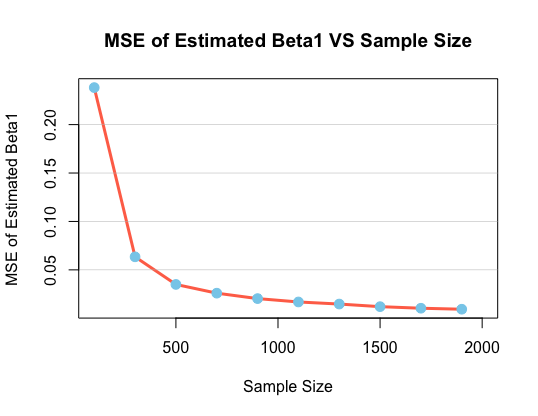
\includegraphics[width=150mm]{mse_samplesize.png}

\noindent This graph shows the MSE of $\hat{\beta}_1$ converges to 0 when sample size increases.

\newpage
\section*{Q2}
\subsection*{Q2-a}
\begin{align*}
\text{the cdf of X is }F_X(x) &= \frac{e^x}{1+e^x} \\
\text{the pdf of X } f_X(x) &= \frac{d F_X}{dx} \\
&= \frac{e^x}{(1 + e^x)^2}
\end{align*}

\noindent Mean of random variable is $\mathbb{E}(X)$
\begin{align*}
\mathbb{E}(X) &= \int_{-\infty}^{\infty} f_X(x) \cdot x \, dx \\
&= - \frac{x}{1 + e^x} + x - \log(e^x + 1) \, |_{-\infty}^{\infty}\\
&= 0 - 0 = 0
\end{align*}

\noindent Median of random variable is the value of $x$ where $F_X(x) = 0.5$
\begin{align*}
\frac{e^x}{1 + e^x} &= 0.5 \\
e^x &= 1 \\
x &= \log(1) = 0
\end{align*}

\noindent Now we get the pdf of random variable $X$ is $\frac{e^x}{(1+e^x)^2}$, and both mean and median equal to 0.


%%% do not touch anything below
\end{document}
